\documentclass[12pt]{article} % Default font size is 12pt, it can be changed here

\usepackage{graphicx} % Required for including pictures
%\usepackage{float} % Allows putting an [H] in \begin{figure} to specify the exact location of the figure
%\usepackage{floatrow}
\usepackage{wrapfig} % Allows in-line images such as the example fish picture
\usepackage[margin=1in, paperwidth=8.5in, paperheight=11in]{geometry}

\linespread{1.2} % Line spacing

\setlength\parindent{0pt} % Uncomment to remove all indentation from paragraphs

\graphicspath{{./Pictures/}} % Specifies the directory where pictures are stored

\date{}

\begin{document}

\title{Pioneer}
\maketitle

\section{Introduction}

Use your technology, resources and military might to expand across the galaxy.

\section{Pieces}

\begin{itemize}
	\item 22x Hexagonal star system tiles
	\item 4x Hexagonal home system tiles
	\item 20x Gold cards
	\item 10x Runite cards
	\item 10x Unobtanium cards
	\item 10x Scout cards
	\item 10x Colonizer cards
	\item 10x Warship cards
	\item 10x Fortification cards
	\item 10x Recycling cards
	\item 10x Tactical Strike cards
	\item 5x Nova Bomb cards
	\item 5x Infinite Improbability Drive cards
	\item 5x Rearden Metal cards
	\item 20x Scout ships, colonizer ships, warships and colonies for each color
	\item 5x Nova bomb pieces
	\item 4x Playmats
	\item 1x Technology board
	\item 1x 6-sided die
\end{itemize}

\section{Starting the Game}

\subsection{Setting up the Star System Board}
First randomly lay out a number of star system tiles face down on the table.  Each must be connected to at least one other tile.  Different numbers of tiles and configurations can be tried based on the number of players and to create different gameplay.  For each player, one of the tiles must be a home system tile, placed face up.  An example board layout for two players is show below:

\centerline{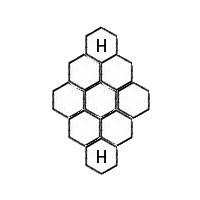
\includegraphics[scale=.75]{hexboard.jpg}}

Each player places one of their colony pieces on a home system tile.  This will be their starting star system.

\subsection{Setting up the Technology Board}

Place a marker for each player in each zero space for the three types of technology - military, transportation and society.

\subsection{Setting up the Cards}

Separate the cards into distinct piles face up on the table.  So there should be a pile for gold, a pile for runite, etc.  Place the Nova Bomb cards on their space on the technology board and then do the same for the Infinite Improbability Drive cards and Rearden Metal cards.  Give each player a play mat which is where they will place their deck and their trash.  Deal each player 5 gold cards.  This will be their initial hand.


\section{Playing the Game}

The game is made up of rounds where each player gets a turn.  Each turn comprises two phases: the card phase, and the board phase.

\subsection{The Card Phase}

During the card phase the player has by default a total of two actions to use.  Actions can be either playing cards from their hand, buying cards from the piles on the table or researching technology.  The actions may be used in any combination of the three ways including doing one twice.

\subsubsection{Buying Cards}

Each card has a price in the upper right hand corner.  This is the amount of money it takes to buy the card.  Money can be gotten in a number of ways.  The primary way is by discarding gold, runite or unobtanium from your hand into the trash pile.  When discarded, each of those cards increases the player's money pool buy the amount specified in the center.  A player may spend up to the amount of money they have in their money pool.  When buying a card, it's price is subtracted from the money pool, and the card goes on top of the player's trash pile.  There are three special cards that are not immediately available for purchase - Nova Bomb, Infinite Improbability Drive and Rearden Metal.  Only once a player has researched to level three in the respective technology area may he purchase those cards.

\subsubsection{Playing Cards}

Actions may also be used to play non-money cards from your hand.  Playing a card takes one action and activates the effect described on the card.  Some cards also cost money to play.  This is signified by the price, and a colon (i.e. "3:") before the description of the effect.  A summary of each effect is described below:

\paragraph{Construct}
Take one of the specified ships and place it onto the board on the same space as one of your colonies.

\paragraph{Fortify}
Take a colony and stack it on top of an existing colony to signify that the colony has been fortified.  This colony now gets bonus attack and defense.

\paragraph{+\$}
Add the specified amount of money to your money pool.

\paragraph{+Action}
Add the number of actions to your action pool.

\paragraph{Draw}
Draw the specified number of cards from your deck.

\subsubsection{Drawing Cards}
Cards are drawn from the top of a player's deck.  If at any time the deck runs out of cards, shuffle the trash and place it face down on the deck zone as the new deck and draw the remainder of the cards from that.

\subsubsection{Researching Technology}
Actions may also be used to research new technology.  There are three areas of technology - military, transportation and society.  Each player starts at level 0 for each area.  To research a technology area, a player may move one of his three markers to the next level for the indicated price.  For example, to move from level 0 military to level 1 military it costs \$5.  Once a player's marker is at an area's technology level, he has access to that level's effect, as well as all lower level's effects.  Level 1 and level 2 effects are passive effects that are always in effect.  Level 3 technologies make special cards available for purchase.  Once an area has been researched to level 3, those cards can be purchased just like any normal card.  Additionally, at the end of the game, players get 5VP for each area they researched to level 3.  Each technology is explained in-depth in the Technologies section.

\subsubsection{Clean Up}
After the player has either used all his actions or decides he doesn't want to use anymore, his card phase is over.  His money pool and action pool empty.  He discards the rest of his hand into his trash pile.  Then draws five new cards.

\subsection{The Board Phase}
After the card phase is over, the board phase begins.  This is when the player can move his pieces around the board, colonize systems and engage in combat.

\subsubsection{Ship Statistics}
Each ship has attack, defense and movement statistics.  These are specified on a chart on each player's play mat.  

\subsubsection{Movement}
Each spaceship may move once per turn a number of spaces equal to the ship's movement statistic.  A ship cannot move through a space occupied by enemies without engaging in combat.

\subsubsection{Scouting}
At the beginning of the game, all the star system tiles are face down with their bonuses hidden.  When a scout ship lands on a tile, a player may peek at the underside of the tile.  He doesn't have to reveal it to anyone else.

\subsubsection{Colonization}
A player may use colonizers to colonize star systems.  When a colonizer lands on a star system that is currently uncolonized, he may remove his colonizer, flip the tile over (if it is still face down) and place a colony on the tile.  While a system is colonized, the player gets the bonuses that the system specified (if any).

\subsubsection{Combat}
When ships move on a tile that contains enemy units (ships or colonies) then there is combat.  Each player adds up the total amount of attack their units have and distribute it in any way across the enemy unit.  If the amount of attack applied to a unit is greater than or equal to the unit's defense, that unit is destroyed at the end of combat.  If the tile contains a colony, the opposing player must first apply enough damage to the his opponents ships to destroy them before applying damage to the colony.  For instance, if Blue has a colony and ships which have a total of 10 defense, and Red is attacking with 12 attack, then 10 of the attack damage must first go to destroying Blue's ships and he can only apply 2 damage to the colony.  After combat, all surviving units remain of the tile.  On future turns, units can move away from a shared tile without initiating combat.

\subsubsection{Star System Bonuses}
All star systems are worth at least 1 Victory Point (VP), but some also provide extra bonuses during the game.  These include extra cards at the beginning of the turn, extra money or extra actions.  At the beginning of a player's turn, he gets the bonuses for any star system he currently has colonized.

\section{Ending the Game}
The game ends when all the star system tiles have been turned face up.  At that time, each player counts up the total number of Victory Points they have for all their currently colonized star systems and from reaching level 3 technologies.  The player with the most victory points is the winner.  To brake a tie, use the following metrics in order: The player with more victory points from technologies, the player with more colonized star systems, the player with more cards in his deck.

\section{Technologies}

\subsection{Military}

\subsubsection{Particle Beam}
Gives all warships you control +1 attack.

\subsubsection{Micro Nuke}
Gives all scouts you control +1 attack.

\subsubsection{Nova Bomb}
The nova bomb allows you to completely destroy a star system.  When playing the nova bomb card, you attach a nova bomb to a scout which is currently on a tile which you have a colony on.  After playing the card, remove it from the game.  When that scout lands on a tile, you may activate the nova bomb instead of scouting or initiating combat.  When activated, all units on the tile, including your own are destroyed.  Furthermore, the nova bomb destroys all the planets in the system and leaves in inhospitable.  Flip the tile over (if it's face down) and leave the nova bomb on the tile to indicate that it can't be colonized again. 

\subsection{Transportation}

\subsubsection{Worm Hole}
Allows your ships to move directly from one tile that you have a colony on to another that you have a colony on.   This uses the ship's move action for the turn.  It cannot be part of another movement.  For example, a scout cannot move 1 tile and then use a wormhole.

\subsubsection{Warpdrive}
Gives all your ships +1 move.

\subsubsection{Infinite Improbability Drive}
When playing an infinite improbability drive, move one of your ships to any other tile on the board.  It can be occupied by enemy units.  Landing effects (i.e. scouting or combat) do not trigger after using this card.  After moving a ship, roll a 6-sided die and get the effect listed on the card which corresponds to the roll of the die.  If a player has no ships, he may not use the dice-rolling effect.

\subsection{Society}

\subsubsection{Robotic Manufacturing}
Gives a player +1 actions per turn.

\subsubsection{Asteroid Mining}
The player draws one extra card at the end of each turn.

\subsubsection{Rearden Metal}
Rearden metal works just like each other metal, expect it gives +\$5.    

\end{document}